\scanpage{137}
% archive foliation: 136
Soit $S$ un schéma \uline{réduit} \uline{connexe}.

On considère des schémas en groupes, finis et plats sur $S$, soit $G$, pour lesquels on a une suite exacte
\diagram{\begin{tikzcd}[column sep=small]
e \arrow[r,no head] & \unsure{U|H} \arrow[r] & G \arrow[r,no head] & \Gamma \arrow[r] & e
\end{tikzcd}}
où la projection $U\to S$ est plate, finie, \deleted{\unsure{s}} et géométriquement \deleted{\unsure{un homéomorphisme}} injectif, et où $\Gamma\unsure{-|\to}S$ est plat, fini, séparable. Alors le sous-$S$-groupe $U$ de $G$ est déterminé de façon unique [pour cette assertion, l'hypothèse ``$S$ réduit'' est-elle nécessaire?].
\margin{\uline{$S$-Groupes} \uline{admissibles} ($S$ réduit?)}
On veut étudier des fibrés principaux \inserted{hom.} $P$ sur de tels $S$-groupes. On suppose $S$ pointé par $a\deleted{\unsure{\xi}}$, et on considère des $P$ avec structure pointée.

\margin{\figure{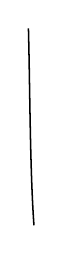
\begin{tikzpicture}\draw[line width=.55pt] (0,2.5) .. controls (.02,1.7) and (.02,.7) .. (.07,0);\end{tikzpicture}}}
\uline{Proposition} \deleted{\unsure{soit $S'\to S$}} Soit $S'\to S$ un morphisme \deleted{plat fini surjectif fidèlement plat}, $G$ un $S$-groupe fini. \deleted{Si $G\times_S S'$ est admissible,} \unsure{?} \inserted{Si $G\deleted{\unsure{\times_S S'}}$ est admissible, $G\times_S S'$ aussi;} la réciproque est vraie si $S'\to S$ est fidèlement plat.
\margin{$S'$ et $S$ réduits}

Direct est trivial. Réciproque résulte de le théorème de la descente et unicité.
